\documentclass[handout,10pt,hyperref={urlcolor=orange}]{beamer}

\usetheme{metropolis}
\usepackage{appendixnumberbeamer}
\usepackage{booktabs}
\usepackage[scale=2]{ccicons}
\usepackage{minted}
%\usepackage{pgfplots}
%\usepgfplotslibrary{dateplot}
\usepackage{hyperref}
\usepackage{graphicx}
\usepackage{xspace}
\newcommand{\themename}{\textbf{\textsc{metropolis}}\xspace}

\title{3D images of buildings in Flanders}
\date{\today}
\author{Quentin Lambotte}
% \titlegraphic{\hfill\includegraphics[height=1.5cm]{logo.pdf}}

\begin{document}

\maketitle

\begin{frame}{Context}
  Build a software that gives a 3D rendering of a building in Flanders, using LiDAR data.

  \begin{figure}[h]
    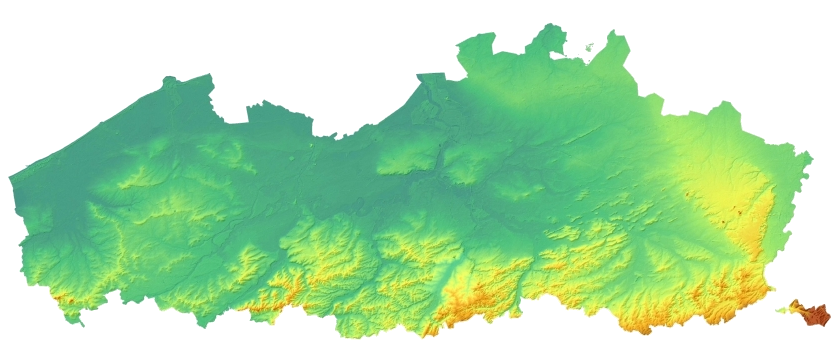
\includegraphics[scale=1]{lidar.png}
    \centering
  \end{figure}
\end{frame}

\begin{frame}{The product}
  The software is available in two versions: one executed unsing a command line and another via a webapp.

  \begin{figure}[h]
    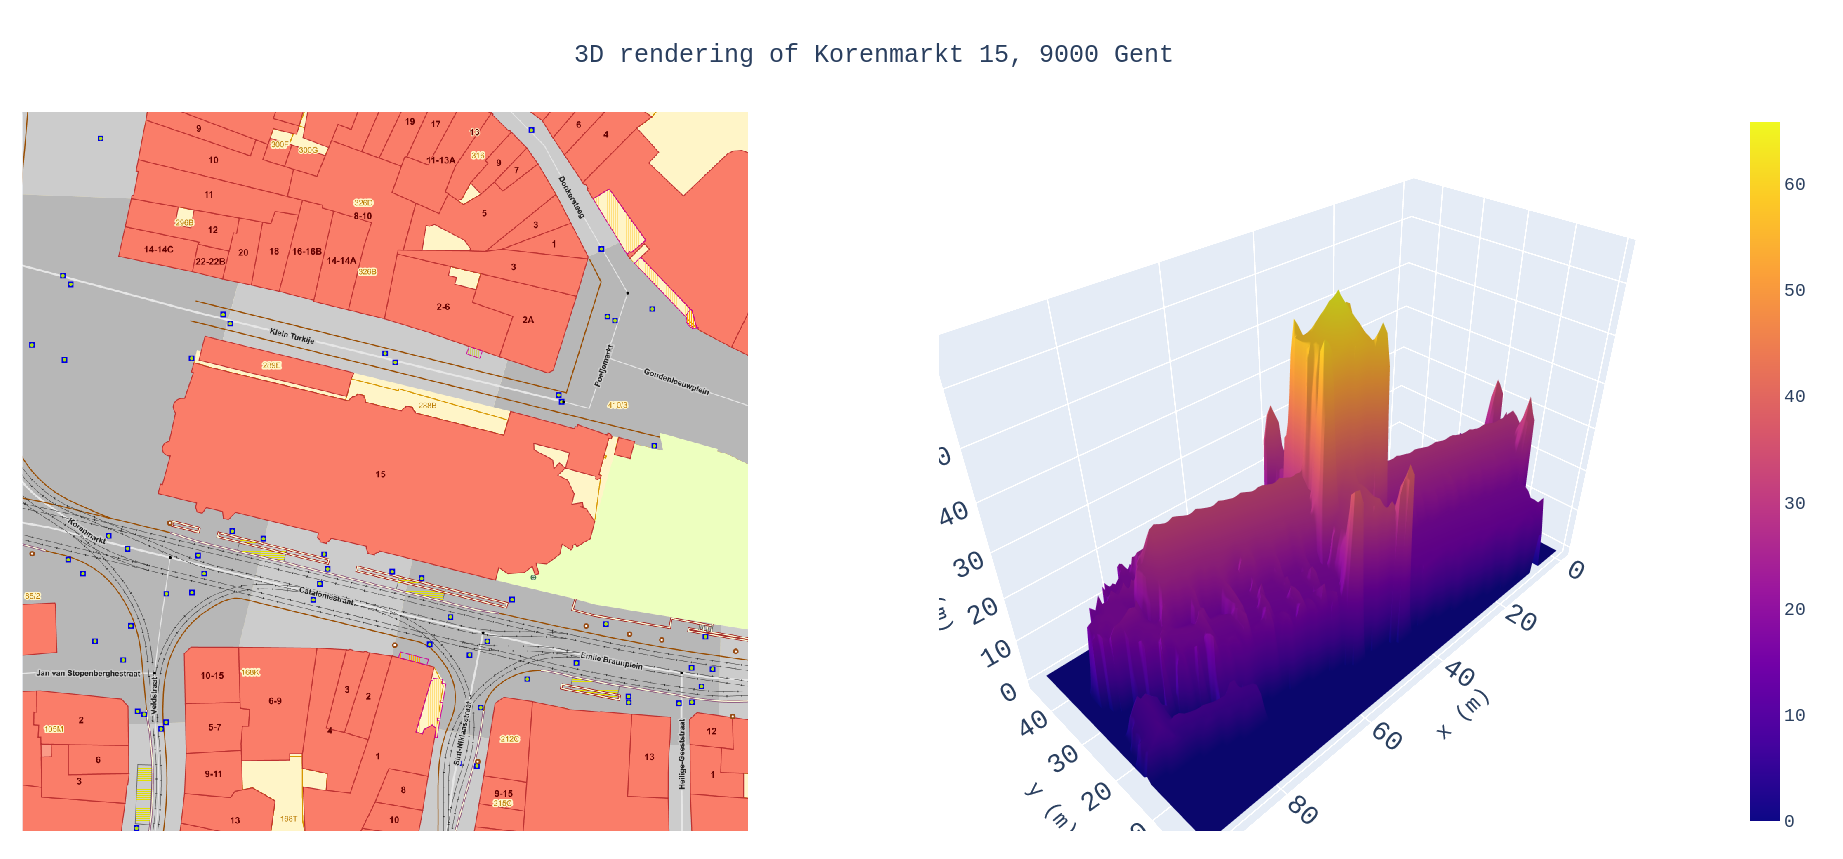
\includegraphics[scale=0.15]{example_t.png}
    \centering
  \end{figure}

\end{frame}
\begin{frame}{Additional features}

  Upon request, the following additional features can be implemented:

  \begin{itemize}
  \item allow user to set options to show a larger area around the building, set the color, add more info on the parcel;
  \item allow to render buildings in brussels and wallonia;
  \item deduce caracteristics of the building and an estimate of the price.
  \end{itemize}

\end{frame}


\end{document}